\cref{fig:additional_figures} shows some additional analyses of the parameter landscape.
\begin{figure*}
  \centering
  \subfloat[Physical runs\label{fig:physical_runs}]{
    \centering
    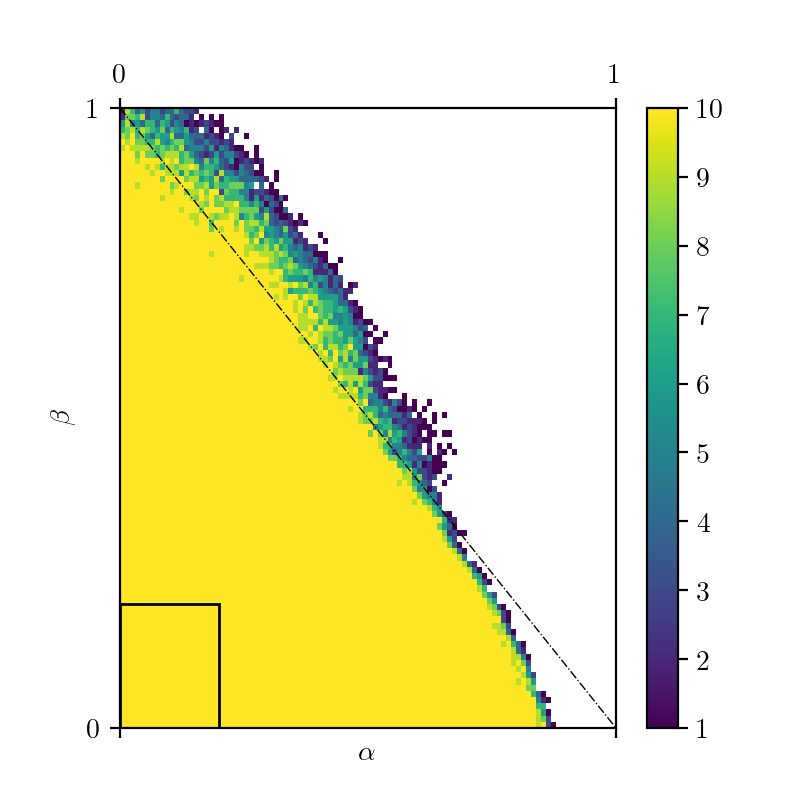
\includegraphics[width=0.32\textwidth]{figure/physical_runs}
  } \hfill
  \subfloat[Chimera variance\label{fig:chimera_var}]{
    \centering
    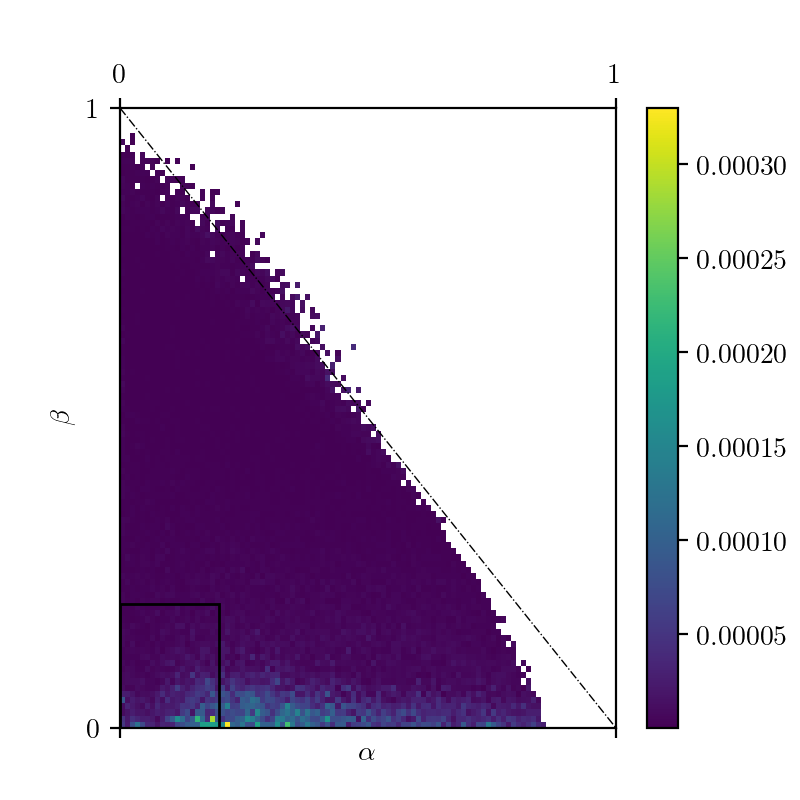
\includegraphics[width=0.32\textwidth]{figure/chimera_var}
  } \hfill
  \subfloat[Metastability\label{fig:meta}]{
    \centering
    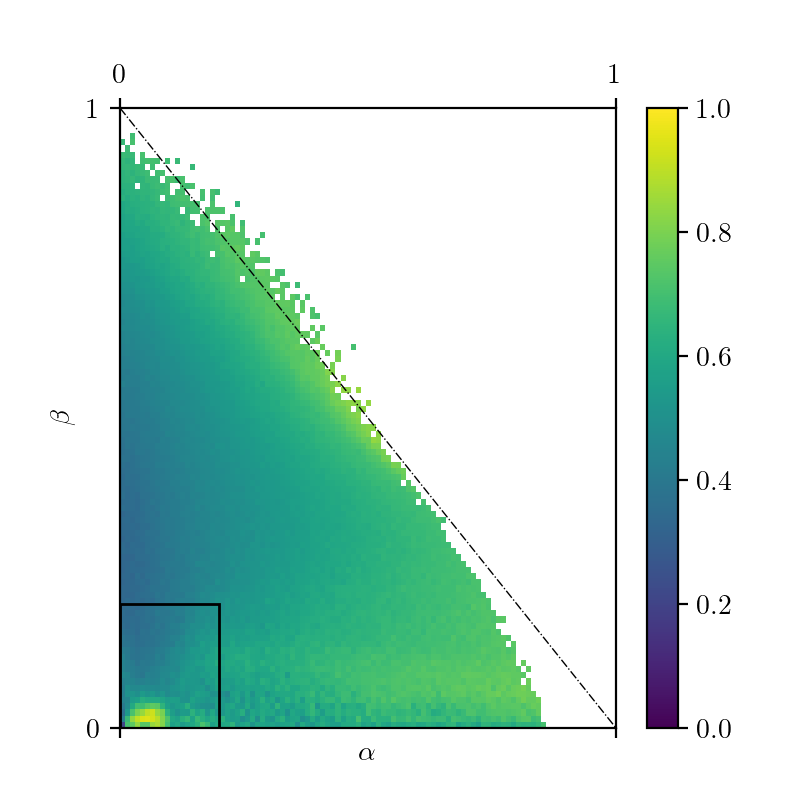
\includegraphics[width=0.32\textwidth]{figure/meta}
  }

  \subfloat[Metastability variance\label{fig:meta_var}]{
    \centering
    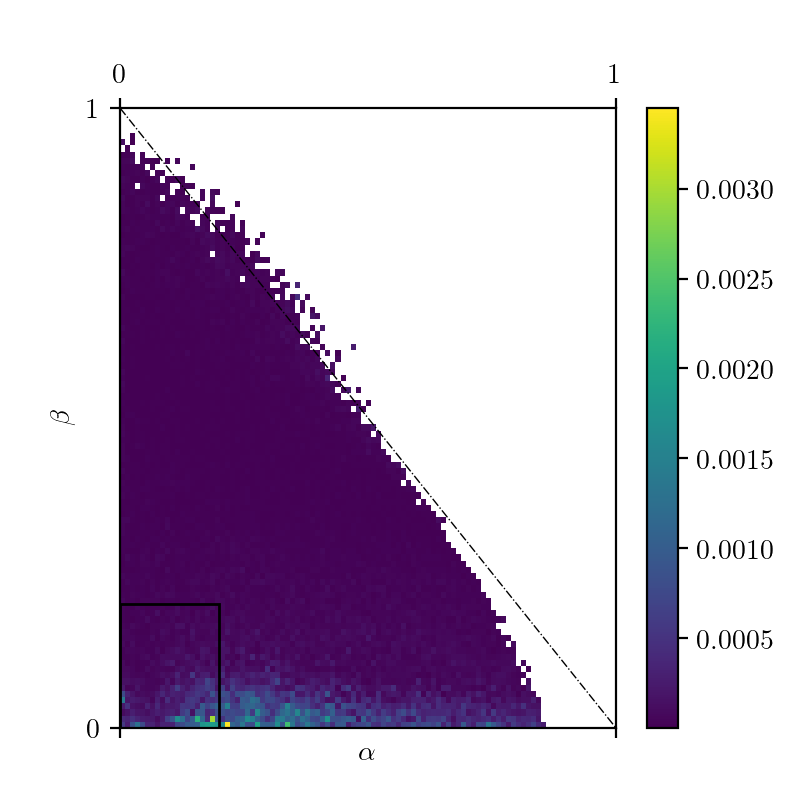
\includegraphics[width=0.32\textwidth]{figure/meta_var}
  } \hfill
  \subfloat[$r$\label{fig:r}]{
    \centering
    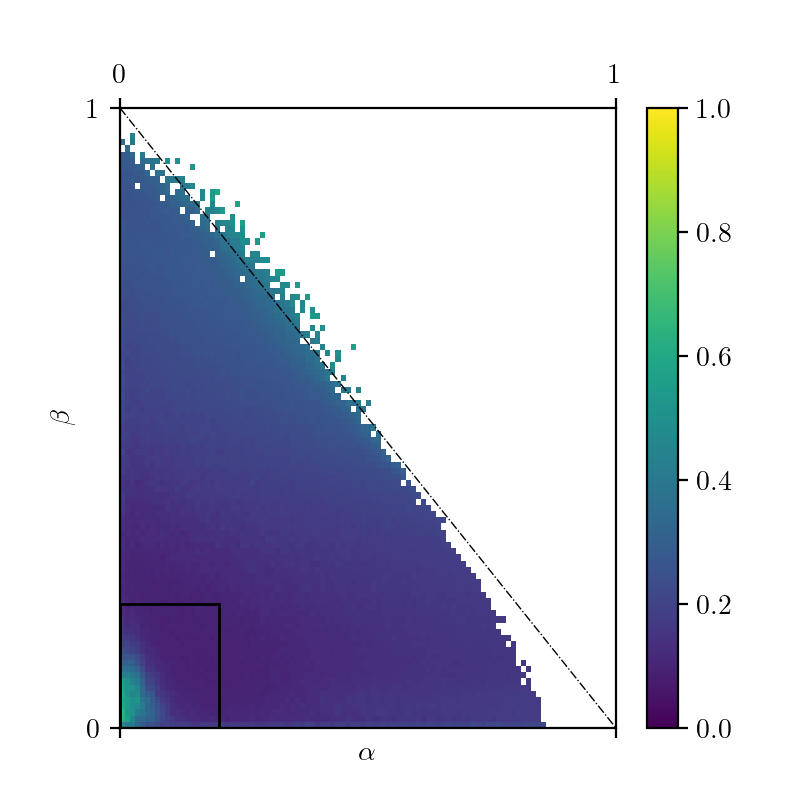
\includegraphics[width=0.32\textwidth]{figure/r}
  } \hfill
  \subfloat[$r$ variance\label{fig:r_var}]{
    \centering
    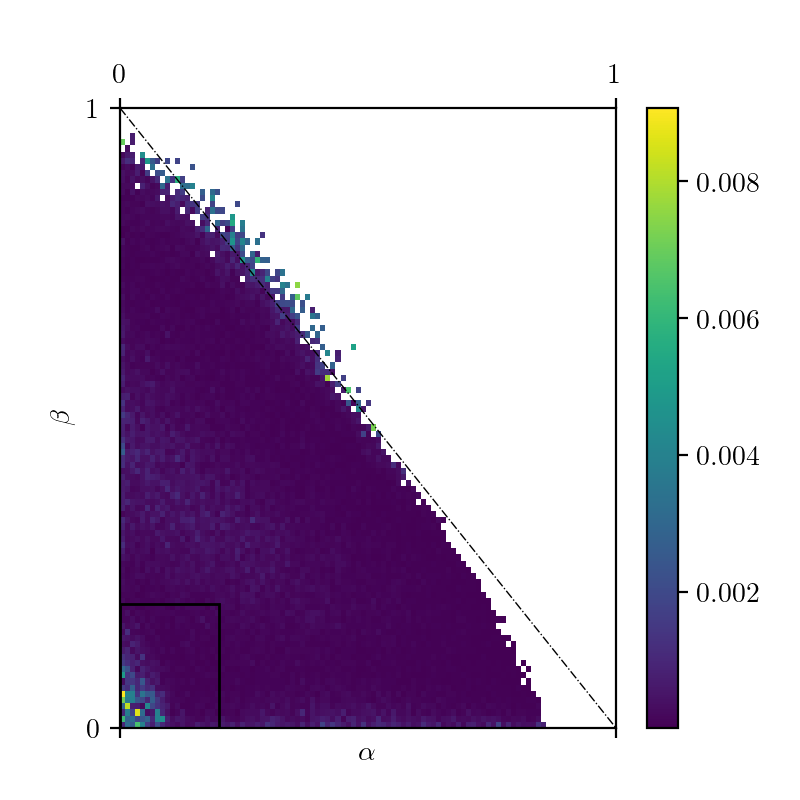
\includegraphics[width=0.32\textwidth]{figure/r_var}
  }
  \caption[Additional figures]{Additional analyses of the parameter landscape.
    \cref{fig:physical_runs} shows the number of runs (out of 10) which gave physical results.
    All parameter sets which are not yellow in \cref{fig:physical_runs} were excluded from the other analyses.
    \cref{fig:chimera_var} shows the variance of the chimera-like index.
    \cref{fig:meta} shows the metastability index.
    \cref{fig:meta_var} shows the variance of the metastability index.
    \cref{fig:r} shows the mean order parameter over time, averaged across runs.
    \cref{fig:r_var} shows the variance between runs of the mean order parameter.
  }
  \label{fig:additional_figures}
\end{figure*}

%%% Local Variables:
%%% mode: latex
%%% TeX-master: "../ms"
%%% End:
